\documentclass[9pt,dvipsnames]{beamer}
\usepackage[T1]{fontenc}
\usepackage{libertinus}
\usepackage{amsmath}
\usepackage[most]{tcolorbox}
\usepackage{graphicx}

\usepackage{hyperref}
\hypersetup{
	colorlinks=true,
}
\usepackage{xcolor}  
\newcommand{\cb}[1]{{\color{CadetBlue}#1}}

\usepackage{pgfplots}
\pgfplotsset{compat=newest}

\setlength{\parskip}{0.5em}

\usepackage{setspace}
\setstretch{1.25}  

\usetheme{Berkeley}
\setbeamertemplate{navigation symbols}{}


\title{CSE574 Introduction to Machine Learning}
\subtitle{Support Vector Machine}
\author{Jue Guo}
\institute{University at Buffalo}
\date{\today}

\begin{document}
\begin{frame}
	\titlepage
\end{frame}


\begin{frame}
	\frametitle{Outline}
	\tableofcontents
\end{frame}



\section{Alternative View of Logistic Regression}
\begin{frame}{Alternative View of Logistic Regression}
	\begin{columns}
		\column{0.5\textwidth}
		A quick review: $h_\theta(x)=\frac{1}{1+e^{-\theta^T x}}$
		\begin{itemize}
			\item if \(y=1\), we want $h_\theta(x) \approx 1$, $\theta^T x \gg 0$
			\item if \(y=0\), we want \(h_\theta(x) \approx 0\), $\theta^T x \ll 0$
		\end{itemize}
		\column{0.5\textwidth}
		\begin{figure}
			\centering
			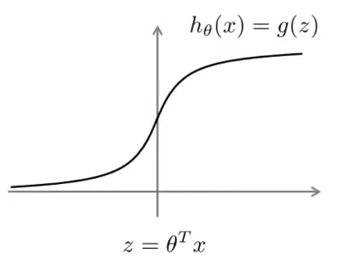
\includegraphics[width=0.9\textwidth]{imgs/svm_1.png}
		\end{figure}

	\end{columns}
	The cost of a single example:

	\begin{align*}
		  & -\left(y \log h_\theta(x)+(1-y) \log \left(1-h_\theta(x)\right)\right)                    \\
		= & -y \log \frac{1}{1+e^{-\theta^T x}}-(1-y) \log \left(1-\frac{1}{1+e^{-\theta^T x}}\right)
	\end{align*}
\end{frame}

\begin{frame}
	\[
		-y \log \frac{1}{1+e^{-\theta^T x}}-(1-y) \log \left(1-\frac{1}{1+e^{-\theta^T x}}\right)
	\]
	\begin{columns}
		\column{0.5\textwidth}
		if \(y=1\) (want $\theta^T x \gg 0$)
		\begin{figure}
			\centering
			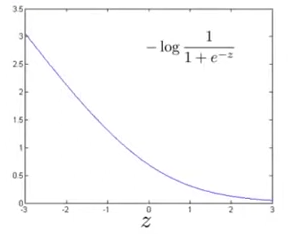
\includegraphics[width=0.7\textwidth]{imgs/svm_2.png}
		\end{figure}
		\column{0.5\textwidth}
		if \(y=0\) (want $\theta^T x \ll 0$)
		\begin{figure}
			\centering
			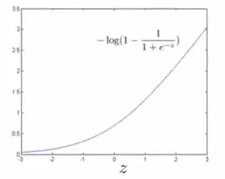
\includegraphics[width=0.7\textwidth]{imgs/svm_3.png}
		\end{figure}
	\end{columns}
\end{frame}

\section{Support Vector Machine}
\begin{frame}{Support Vector Machine}
	\textbf{Cost Function of Logistic Regression}
	\begin{align*}
		\min _\theta \frac{1}{m}\Bigg[ & \sum_{i=1}^m y^{(i)}\left(-\log h_\theta\left(x^{(i)}\right)\right)\\
		                               & + \left(1-y^{(i)}\right)\left(-\log \left(1-h_\theta\left(x^{(i)}\right)\right)\right)\Bigg] \\
		                               & + \frac{\lambda}{2 m} \sum_{j=1}^n \theta_j^2
	\end{align*}
	\textbf{Cost Function of Support Vector Machine}
	$$
		\min _\theta C \sum_{i=1}^m\left[y^{(i)} \operatorname{cost}_1\left(\theta^T x^{(i)}\right)+\left(1-y^{(i)}\right) \operatorname{cost}_0\left(\theta^T x^{(i)}\right)\right]+\frac{1}{2} \sum_{i=1}^n \theta_j^2
	$$
\end{frame}

\subsection{Large Margin Intuition}
\begin{frame}{Large Margin Intuition}
	\textbf{Support Vector Machine}
	$$
		\min _\theta C \sum_{i=1}^m\left[y^{(i)} \operatorname{cost}_1\left(\theta^T x^{(i)}\right)+\left(1-y^{(i)}\right) \operatorname{cost}_0\left(\theta^T x^{(i)}\right)\right]+\frac{1}{2} \sum_{i=1}^n \theta_j^2
	$$
	\begin{columns}
		\column{0.5\textwidth}
		\begin{figure}
			\centering
			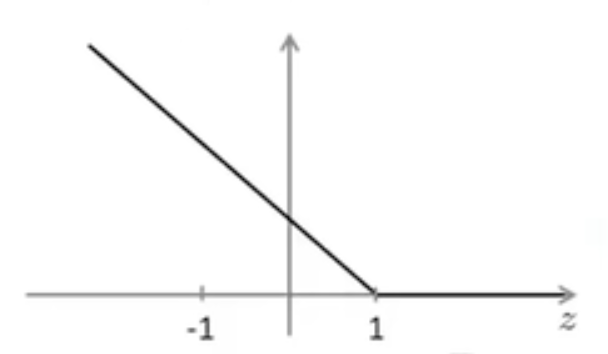
\includegraphics[width=\textwidth]{imgs/svm_4.png}
		\end{figure}
		If \(y=1\), we want \(\theta^{T} x \geq 1\) (not just \(\left.\geq 0\right)\)
		
		\column{0.5\textwidth}
		\begin{figure}
			\centering
			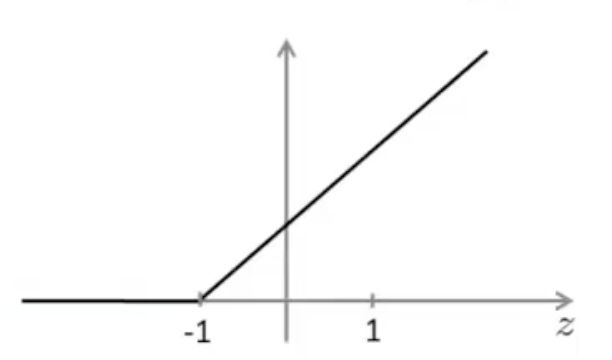
\includegraphics[width=\textwidth]{imgs/svm_5.png}
		\end{figure}
		If \(y=0\), we want \(\theta^{T} x \leq-1\) (not just \(\left.<0\right)\)
	\end{columns}
\end{frame}

\begin{frame}{A very large \(C\)}
	\textbf{Support Vector Machine}
	$$
	\min _\theta C \sum_{i=1}^m\left[y^{(i)} \operatorname{cost}_1\left(\theta^T x^{(i)}\right)+\left(1-y^{(i)}\right) \operatorname{cost}_0\left(\theta^T x^{(i)}\right)\right]+\frac{1}{2} \sum_{i=1}^n \theta_j^2
	$$
	Given that \(C\) is a very large value, we want that the first term to be \(0\). Let's try to understand the optimization problem in the context of what would it take to make this first term in the objective equal to \(0\). 
	\vspace{0.3cm}
	\begin{columns}
		\column{0.5\textwidth}
		Whenever \(y^{(i)}=1\), \(\theta^{\top} x^{(i)} \geqslant 1\); 
		\column{0.5\textwidth}
		Whenever \(y^{(i)}=0\), \(\theta^{\top} x^{(i)} \leqslant-1\)
	\end{columns}
	
	Now, the optimization problem can be written as: 
	\begin{equation*}
		\begin{aligned}
			& \text{min} C\cdot 0 + \frac{1}{2}\sum_{i=1}^n \theta_j^2 \\
			\text{s.t.  } &  \theta^{\top} x^{(i)} \geqslant 1 \quad \text { if } y^{(i)}=1 \\
			& \theta^{T} x^{(i)} \leqslant-1 \quad \text {if } y^{(i)}=0
		\end{aligned}
	\end{equation*}
\end{frame}

\begin{frame}
	\textbf{SVM Decision Boundary: Linearly separable case}
\begin{figure}
	\centering
	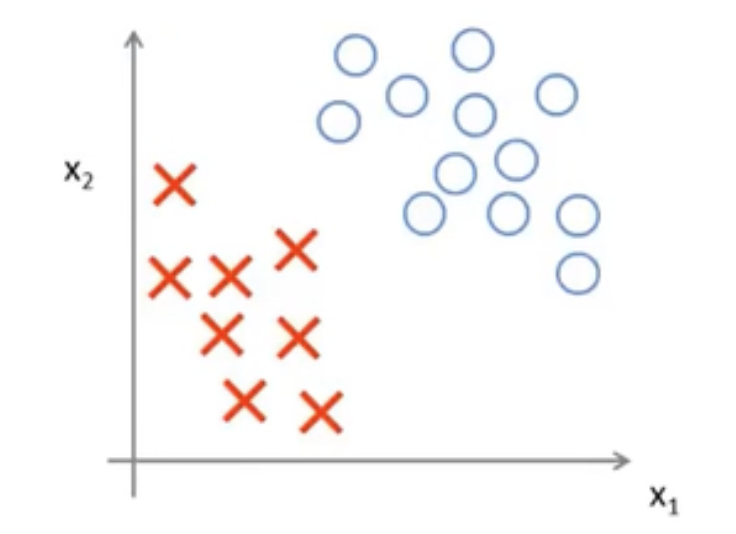
\includegraphics[width=0.4\linewidth]{imgs/svm_6}
	\caption{Linearly Separable Case}
	\label{fig:svm6}
\end{figure}
\end{frame}

\begin{frame}
	\textbf{Large margin classifier in presence of outliers}
	\begin{figure}
		\centering
		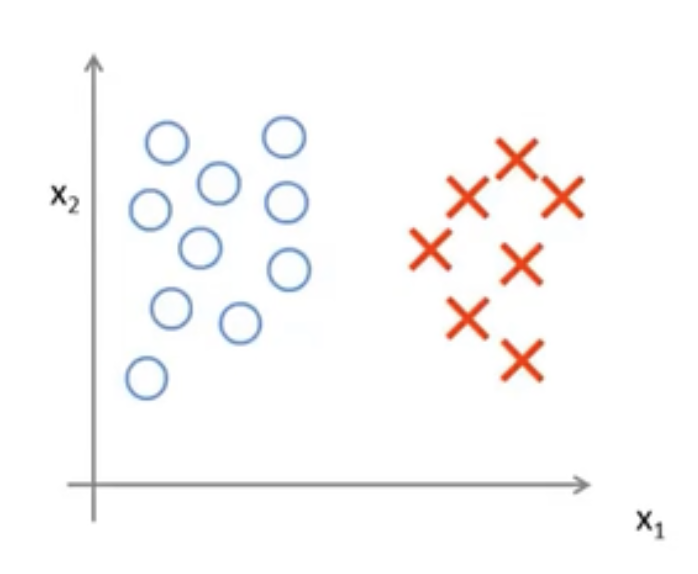
\includegraphics[width=0.4\linewidth]{imgs/svm_7}
		\label{fig:svm7}
	\end{figure}
\end{frame}

\subsection{The Mathematics behind Large Margin Classification}
\begin{frame}{The Mathematics behind Large Margin Classification}
	\textbf{Vector Inner Product}
	\vspace{0.5cm}
	\begin{columns}[T]
		\column{0.5\textwidth}
		\begin{tikzpicture}[scale=0.7] % Adjust the scale to make the plot smaller
			\begin{axis}[
				axis lines=middle,
				axis line style={->},
				xlabel={$x$},
				ylabel={$y$},
				xlabel style={at={(ticklabel* cs:1)},anchor=west},
				ylabel style={at={(ticklabel* cs:1)},anchor=south},
				xmin=0, xmax=5, % Only positive x-axis
				ymin=0, ymax=5, % Only positive y-axis
				ticks=none,
				small,
				]
			\end{axis}
		\end{tikzpicture}
				\begin{tikzpicture}[scale=0.7] % Adjust the scale to make the plot smaller
			\begin{axis}[
				axis lines=middle,
				axis line style={->},
				xlabel={$x$},
				ylabel={$y$},
				xlabel style={at={(ticklabel* cs:1)},anchor=west},
				ylabel style={at={(ticklabel* cs:1)},anchor=south},
				xmin=0, xmax=5, % Only positive x-axis
				ymin=0, ymax=5, % Only positive y-axis
				ticks=none,
				small,
				]
			\end{axis}
		\end{tikzpicture}
		\column{0.5\textwidth}
		$u=\left[\begin{array}{l}u_{1} \\ u_{2}\end{array}\right] \quad v=\left[\begin{array}{l}v_{1} \\ v_{2}\end{array}\right]$
	\end{columns}
\end{frame}

\begin{frame}{SVM Decision Boundary}
	\begin{columns}[T]
	    \column{0.5\textwidth}
		\begin{align*}
			\min_{\theta} \quad & \frac{1}{2} \sum_{j=1}^{n} \theta_{j}^{2} \\
			\text{s.t.} \quad & \theta^{T} x^{(i)} \geq 1 \quad \text{if } y^{(i)}=1 \\
			& \theta^{T} x^{(i)} \leq -1 \quad \text{if } y^{(i)}=0
		\end{align*}
		\column{0.5\textwidth}
		\begin{tikzpicture}[scale=0.7] % Adjust the scale to make the plot smaller
		\begin{axis}[
			axis lines=middle,
			axis line style={->},
			xlabel={$x$},
			ylabel={$y$},
			xlabel style={at={(ticklabel* cs:1)},anchor=west},
			ylabel style={at={(ticklabel* cs:1)},anchor=south},
			xmin=0, xmax=5, % Only positive x-axis
			ymin=0, ymax=5, % Only positive y-axis
			ticks=none,
			small,
			]
		\end{axis}
		\end{tikzpicture}
	\end{columns}
\end{frame}

\begin{frame}
\begin{align*}
	\min_{\theta} \quad & \frac{1}{2} \sum_{j=1}^{n} \theta_{j}^{2} =\frac{1}{2}\|\theta\|^{2} \\
	\text{s.t.} \quad & p^{(i)} \cdot \|\theta\| \geq 1 \quad \text{if } y^{(i)}=1 \\
	& p^{(i)} \cdot \|\theta\| \leq -1 \quad \text{if } y^{(i)}=0
\end{align*}
where \(p^{(i)}\) is the projection of \(x^{(i)}\) onto the vector \(\theta\).
Simplification: \(\theta_{0}=0\); this simplification merely makes the decision boundary to pass through (0,0);
\vspace{0.3cm}
\begin{columns}
	\column{0.5\textwidth}
	\textbf{Bad Decision Boundary}
	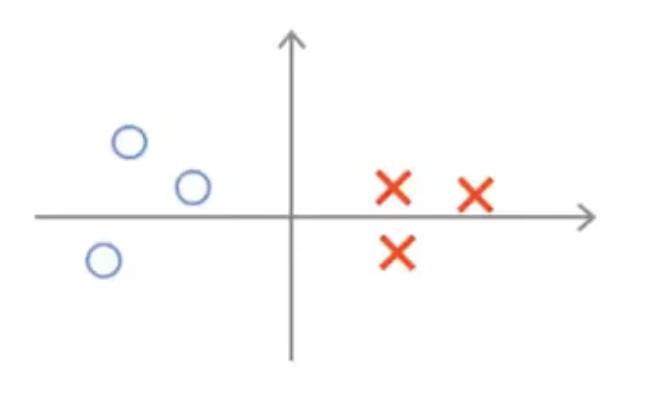
\includegraphics[width = \textwidth]{imgs/svm_8.png}
	\column{0.5\textwidth}
	\textbf{Good Decision Boundary}
	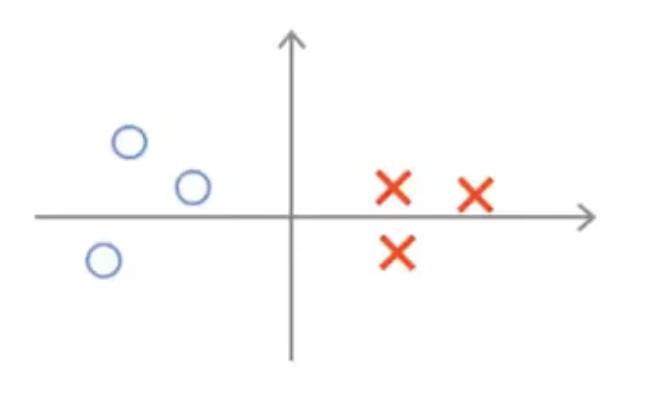
\includegraphics[width = \textwidth]{imgs/svm_8.png}
\end{columns}
\end{frame}

\begin{frame}{Reading Assignments}
	\begin{enumerate}
		\item Why the parameter vector orthogonal to the decision boundary?
		\begin{itemize}
			\item \href{https://stackoverflow.com/questions/10177330/why-is-weight-vector-orthogonal-to-decision-plane-in-neural-networks/10357067}{Orthogonality in Neural Network}
			\item 			\href{https://datascience.stackexchange.com/questions/6054/in-svm-algorithm-why-vector-w-is-orthogonal-to-the-separating-hyperplane}{SVM}
		\end{itemize}
	\end{enumerate}
\end{frame}

\section{Kernels}
\begin{frame}{Non-linear Decision Boundary}
	\begin{columns}[T]
		\column{0.4\textwidth}
		\begin{figure}
			\centering
			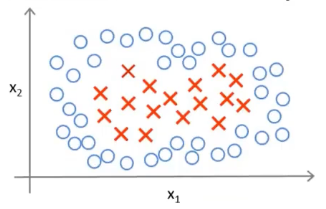
\includegraphics[width=\textwidth]{imgs/svm_9.png}
		\end{figure}
		\column{0.6\textwidth}
		Predict \(y=1\) if 
		\vspace{0.3cm}
		
		\(\theta_{0}+\theta_{1} x_{1}+\theta_{2} x_{2}+\theta_{3} x_{1} x_{2}+\theta_{4} x_{1}^{2}+\theta_{5} x_{2}^{2}+\cdots \geq 0\)
		
		 $$
		 h_{0}(x)=\left\{\begin{array}{ll}1 & \text { if } \theta_{0}+\theta_{1} x_{1}+\cdots \geqslant 0 \\ 0 & \text { otherise. }\end{array}\right.
		 $$
		 
		\begin{align*}
			\theta_{0} & +\theta_{1} f_{1} + \theta_{2} f_{2} + \theta_{3} f_{3} + \cdots \\
			f_{1} & =x_{1}, \quad f_{2}=x_{2}, \quad f_{3}=x_{1} x_{2}, \\
			f_{4} & =x_{1}^{2}, \quad f_{5}=x_{2}^{2}, \ldots
		\end{align*}
	\end{columns}
	\vspace{0.3cm}
	Is there a different/ better choice of the features \(f_{1}, f_{2}, f_{3}, \ldots\)?
\end{frame}

\begin{frame}{Kernel}
	\begin{columns}[T]
		\column{0.4\textwidth}
				\begin{tikzpicture}[scale=0.7] % Adjust the scale to make the plot smaller
			\begin{axis}[
				axis lines=middle,
				axis line style={->},
				xlabel={$x_1$},
				ylabel={$x_2$},
				xlabel style={at={(ticklabel* cs:1)},anchor=west},
				ylabel style={at={(ticklabel* cs:1)},anchor=south},
				xmin=0, xmax=5, % Only positive x-axis
				ymin=0, ymax=5, % Only positive y-axis
				ticks=none,
				small,
				]
			\end{axis}
		\end{tikzpicture}
		\column{0.6\textwidth}
		Given \(x\), compute new feature depending on proximity to landmarks \(l^{(1)}, l^{(2)}, l^{(3)}\); 
		
		\textcolor{red}{Given \(x\)}:
		\begin{itemize}
			\item  \(f_1 = \text{similarity}(x,l^{(1)})\) = \(\text{exp}(-\frac{\left\|x-l^{(1)}\right\|^{2}}{2\sigma^{2}})\)
			\item \(f_2 = \text{similarity}(x,l^{(2)})\) = \(\text{exp}(-\frac{\left\|x-l^{(2)}\right\|^{2}}{2\sigma^{2}})\)
			\item  \(f_3 = \text{similarity}(x,l^{(3)})\) = \(\text{exp}(...)\)
		\end{itemize}
		
	\end{columns}
\end{frame}

\begin{frame}{Kernel and Similarity}
	$$
	f_{1}=\operatorname{similarity}\left(x, l^{(1)}\right)=\exp \left(-\frac{\left\|x-l^{(1)}\right\|^{2}}{2 \sigma^{2}}\right)= \exp \left(-\frac{\sum_{j=1}^{n}\left(x_{j}-l_{j}^{(1)}\right)^{2}}{2 \sigma^{2}}\right)
	$$
	\begin{itemize}
		\item if \(x \approx l^{(1)}\): \(f_{1} \approx \exp \left(-\frac{0^{2}}{2 \sigma^{2}}\right)\approx 1\)
		\item If \(x\) if far from \(l^{(1)}\): \(f_{1}=\exp \left(-\frac{(\text { large number })^{2}}{2\sigma^{2}}\right) \approx 0\)
	\end{itemize}
\end{frame}

\begin{frame}{Example and Affects of \(\sigma\)}
	$$
	l^{(1)}=\left[\begin{array}{l}3 \\ 5\end{array}\right], \quad f_{1}=\exp \left(-\frac{\left\|x-l^{(1)}\right\|^{2}}{2 \sigma^{2}}\right)
	$$
	\begin{columns}[T]
		\column{0.5\textwidth}
		$$\sigma^{2}=1$$
		\begin{figure}
			\centering
			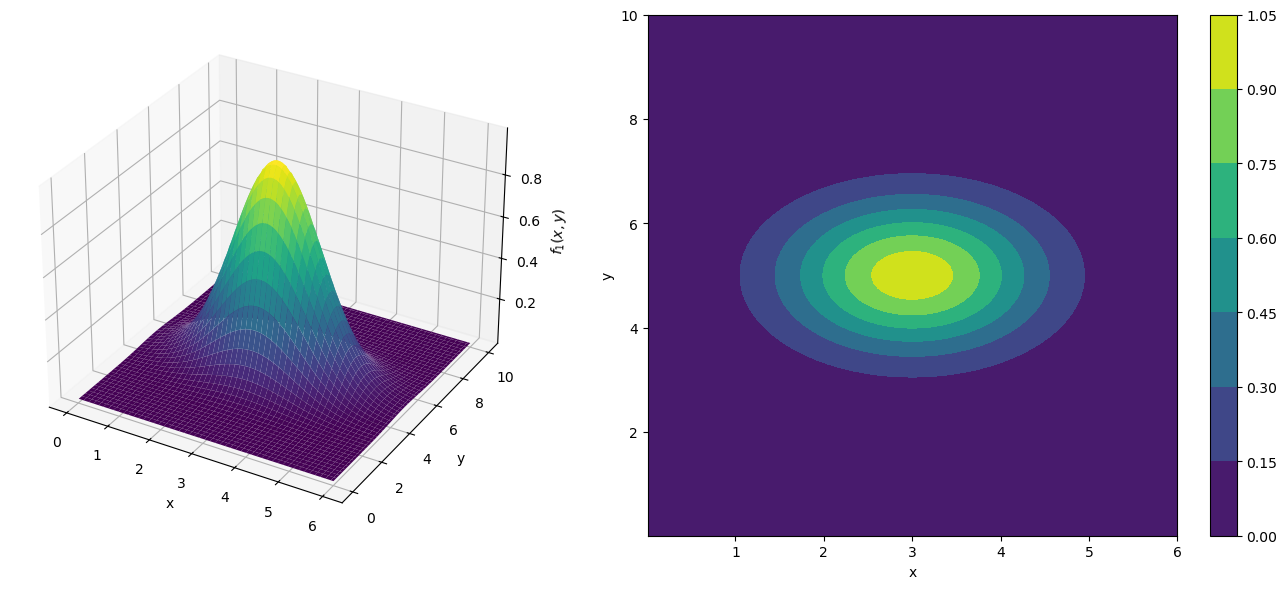
\includegraphics[width=\textwidth]{imgs/svm_10.png}
		\end{figure}
		When \(x=\left[\begin{array}{l}3 \\ 5\end{array}\right]\), you will get \(f_{1}=1\); It basically measures how close are you to the landmark.
		\column{0.5\textwidth}
		$$\sigma^{2}=0.5$$
		\begin{figure}
			\centering
			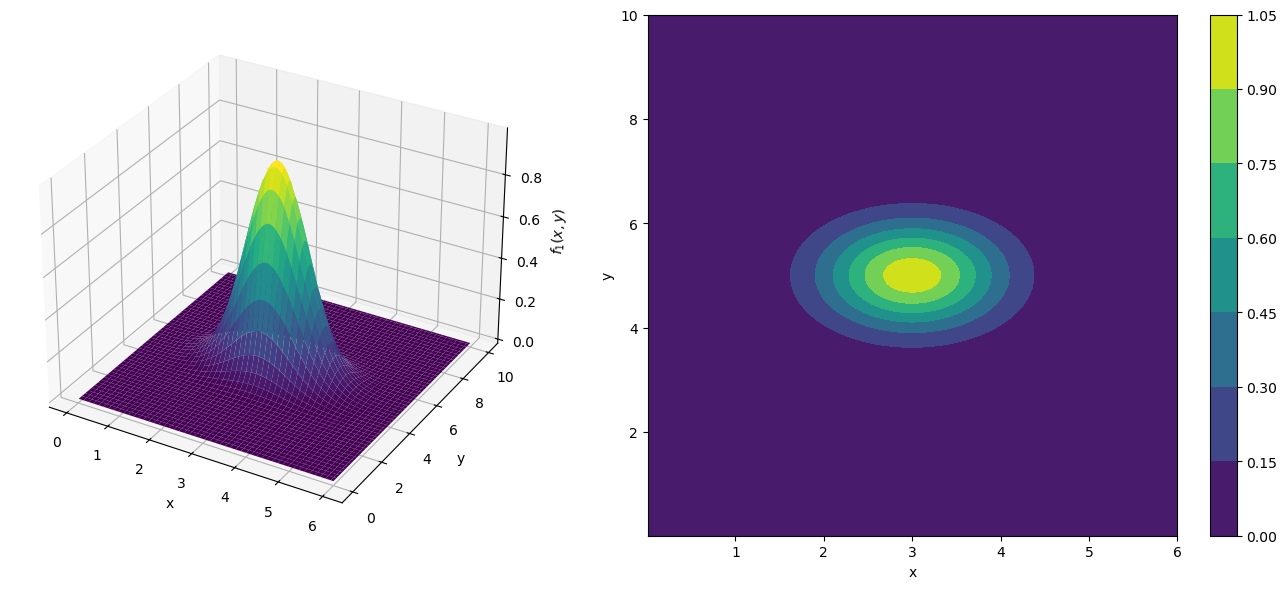
\includegraphics[width=\textwidth]{imgs/svm_11.png}
		\end{figure}
		The width of the bump become narrower, and width of contour; The feature \(f_{1}\) falls to zero more rapidly; 
	\end{columns}
\end{frame}

\begin{frame}
	\begin{columns}[T]
		\column{0.5\textwidth}
		\begin{tikzpicture}[scale=0.5]
			\begin{axis}[
				axis lines=middle,
				xlabel={$x_1$},
				ylabel={$x_2$},
				xlabel style={at={(ticklabel* cs:1)},anchor=north},
				ylabel style={at={(ticklabel* cs:1)},anchor=east},
				xmin=0, xmax=5,
				ymin=0, ymax=5,
				ticks=none
				]
				
				% Add the points
				\addplot[only marks, mark=*, blue] coordinates {(1,4) (4,3) (3,1)};
				
				% Add the labels
				\node[label={180:{$l^{(1)}$}},circle,fill,inner sep=2pt] at (axis cs:1,4) {};
				\node[label={180:{$l^{(2)}$}},circle,fill,inner sep=2pt] at (axis cs:4,3) {};
				\node[label={180:{$l^{(3)}$}},circle,fill,inner sep=2pt] at (axis cs:3,1) {};
				
			\end{axis}
		\end{tikzpicture}
		\column{0.5\textwidth}
		Given a training example \(x\); 
		
		\textcolor{red}{Hypothesis:} Predict " 1 " when \(\theta_{0}+\theta_{1} f_{1}+\theta_{2} f_{2}+\theta_{3} f_{3} \geq 0\)
		
		\textbf{Assume} that we already have our model: \(\theta_{0}=-0.5, \theta_{1}=1, \theta_{2}=1, \theta_{3}=0\)
	\end{columns}
\end{frame}

\begin{frame}
	\begin{columns}[T]
		\column{0.5\textwidth}
		\begin{tikzpicture}[scale=0.5]
			\begin{axis}[
				axis lines=middle,
				xlabel={$x_1$},
				ylabel={$x_2$},
				xlabel style={at={(ticklabel* cs:1)},anchor=north},
				ylabel style={at={(ticklabel* cs:1)},anchor=east},
				xmin=0, xmax=5,
				ymin=0, ymax=5,
				ticks=none
				]
				
				% Add the points
				\addplot[only marks, mark=*, blue] coordinates {(1,4) (4,3) (3,1)};
				\addplot[only marks, mark=*, red] coordinates {(1.2,3.8)};
				
				% Add the labels
				\node[label={180:{$l^{(1)}$}},circle,fill,inner sep=2pt] at (axis cs:1,4) {};
				\node[label={180:{$l^{(2)}$}},circle,fill,inner sep=2pt] at (axis cs:4,3) {};
				\node[label={180:{$l^{(3)}$}},circle,fill,inner sep=2pt] at (axis cs:3,1) {};
				\node[label={270:{$x$}},circle,fill,inner sep=2pt] at (axis cs:1.2,3.8) {};
				
			\end{axis}
		\end{tikzpicture}
		\column{0.5\textwidth}
		Given a training example \(x\); 
		
		\textcolor{red}{Hypothesis:} Predict " 1 " when \(\theta_{0}+\theta_{1} f_{1}+\theta_{2} f_{2}+\theta_{3} f_{3} \geq 0\)
		
		\textbf{Assume} that we already have our model: \(\theta_{0}=-0.5, \theta_{1}=1, \theta_{2}=1, \theta_{3}=0\)
	\end{columns}
	
	\(f_1\approx1, f_2\approx0\) and \(f_3\approx0\);  \(\theta_{0}+\theta_{1}\times 1 + \theta_{2}\times 0 + \theta_{3}\times 0 = -0.5 + 1 = 0.5 \geq 0 \); therefore, we classify this \(x\) as 1. 
\end{frame}

\begin{frame}
	\begin{columns}
		\column{0.5\textwidth}
			\begin{tikzpicture}[scale=0.5]
			\begin{axis}[
				axis lines=middle,
				xlabel={$x_1$},
				ylabel={$x_2$},
				xlabel style={at={(ticklabel* cs:1)},anchor=north},
				ylabel style={at={(ticklabel* cs:1)},anchor=east},
				xmin=0, xmax=5,
				ymin=0, ymax=5,
				ticks=none
				]
				
				% Add the points
				\addplot[only marks, mark=*, blue] coordinates {(1,4) (4,3) (3,1)};
				\addplot[only marks, mark=*, red] coordinates {(4,1)};
				
				% Add the labels
				\node[label={180:{$l^{(1)}$}},circle,fill,inner sep=2pt] at (axis cs:1,4) {};
				\node[label={180:{$l^{(2)}$}},circle,fill,inner sep=2pt] at (axis cs:4,3) {};
				\node[label={180:{$l^{(3)}$}},circle,fill,inner sep=2pt] at (axis cs:3,1) {};
				\node[label={270:{$x$}},circle,fill,inner sep=2pt] at (axis cs:4,1) {};
				
			\end{axis}
		\end{tikzpicture}
		\column{0.5\textwidth}
		\(f_{1}, f_{2}, f_{3} \approx 0\); \(\theta_{0}+\theta_{1} f_{1}+\ldots \approx-0.5\)
		
		With the definition of \textit{landmarks} and \textit{kernel function} , we can learn pretty complex non-linear decision boundaries. 
		\begin{enumerate}
			\item How to decide these landmarks? 
			\item Other similarity functions?
		\end{enumerate}
	\end{columns}
\end{frame}

\begin{frame}{Choosing the Landmarks}
	\begin{columns}
		\column{0.5\textwidth}
		\begin{tikzpicture}[scale=0.5]
			\begin{axis}[
				axis lines=middle,
				xlabel={$x_1$},
				ylabel={$x_2$},
				xlabel style={at={(ticklabel* cs:1)},anchor=north},
				ylabel style={at={(ticklabel* cs:1)},anchor=east},
				xmin=0, xmax=5,
				ymin=0, ymax=5,
				ticks=none
				]
				
				% Add the points
				\addplot[only marks, mark=*, blue] coordinates {(1,4) (4,3) (3,1)};
				
				% Add the labels
				\node[label={180:{$l^{(1)}$}},circle,fill,inner sep=2pt] at (axis cs:1,4) {};
				\node[label={180:{$l^{(2)}$}},circle,fill,inner sep=2pt] at (axis cs:4,3) {};
				\node[label={180:{$l^{(3)}$}},circle,fill,inner sep=2pt] at (axis cs:3,1) {};
				
			\end{axis}
		\end{tikzpicture}
		\column{0.5\textwidth}
		Given \(x\) :
		$$
		\begin{aligned} f_{i} & =\operatorname{similarity}\left(x, l^{(i)}\right) \\ & =\exp \left(-\frac{\left\|x-l^{(i)}\right\|^{2}}{2 \sigma^{2}}\right)\end{aligned}
		$$
	\end{columns}
	Predict \(y=1\) if \(\theta_{0}+\theta_{1} f_{1}+\theta_{2} f_{2}+\theta_{3} f_{3} \geq 0\); 
	Where to get \(l^{(1)}, l^{(2)}, l^{(3)}, \ldots\) ?
\end{frame}

\begin{frame}
	\begin{columns}
		\column{0.5\textwidth}
		\begin{center}
			\begin{tikzpicture}[scale=0.5]
				\begin{axis}[
					axis lines=middle,
					xmin=0, xmax=10,
					ymin=0, ymax=10,
					ticks=none,
					axis equal image, % Keeps the aspect ratio of the axes the same
					]
					
					% Add red crosses
					\addplot[only marks, mark=x, red, mark size=6pt] coordinates {
						(3,4) (4,3) (5,5) (6,4) (7,3)
					};
					
					% Add blue circles, with increased size to ensure they enclose the red crosses
					\addplot[only marks, mark=o, blue, mark size=6pt] coordinates {
						(3,6) (1,4) (1, 2) (2,1) (7,4) (6, 6) (6,2)
					};
					
				\end{axis}
			\end{tikzpicture}
		\end{center}

		\column{0.5\textwidth}
		\begin{center}
			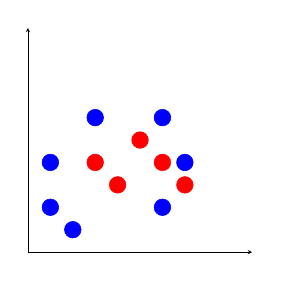
\begin{tikzpicture}[scale=0.5]
				\begin{axis}[
					axis lines=middle,
					xmin=0, xmax=10,
					ymin=0, ymax=10,
					ticks=none,
					axis equal image, % Keeps the aspect ratio of the axes the same
					]
					
					% Add red crosses
					\addplot[only marks, red, mark size=6pt] coordinates {
						(3,4) (4,3) (5,5) (6,4) (7,3)
					};
					
					% Add blue circles, with increased size to ensure they enclose the red crosses
					\addplot[only marks, blue, mark size=6pt] coordinates {
						(3,6) (1,4) (1, 2) (2,1) (7,4) (6, 6) (6,2)
					};
					
				\end{axis}
			\end{tikzpicture}
		\end{center}

	\end{columns}
\end{frame}

\begin{frame}{SVM with Kernels}
	\textcolor{red}{Given} \(\left(x^{(1)}, y^{(1)}\right),\left(x^{(2)}, y^{(2)}\right), \ldots,\left(x^{(m)}, y^{(m)}\right)\), choose \(l^{(1)}=x^{(1)}, l^{(2)}=x^{(2)}, \ldots, l^{(m)}=x^{(m)}\)
	
	\textcolor{red}{Given} example \(x\) :
	$$
	\begin{array}{l}f_{1}=\operatorname{similarity}\left(x, l^{(1)}\right) \\ f_{2}=\operatorname{similarity}\left(x, l^{(2)}\right) \\ \ldots\end{array} \rightarrow 
	f=\left[\begin{array}{c}f_{1} \\ f_{2} \\ \vdots \\ f_{m}\end{array}\right]
	$$
	\end{frame}
	
	\begin{frame}
		For training example \(\left(x^{(i)}, y^{(i)}\right)\):
		$$
		\begin{aligned} f_{1}^{(i)} & =\text{sim} \left(x^{(i)}, l^{(1)}\right) \\ x^{(i)} \rightarrow \quad f_{2}^{(i)} & =\text{sim} \left(x^{(i)}, l^{(2)}\right) \\ \vdots \\ f_{i}^{(i)}& =\text{sim} \left(x^{(i)}, l^{(i)}\right)=\exp \left(-\frac{0}{2\sigma^2}\right)=1 \\ \vdots & \\ f_{m}^{(i)} & =\text{sim} \left(x^{(i)}, l^{(m)}\right)\end{aligned}
		$$
\end{frame}
	
\begin{frame}
	\textcolor{red}{Hypothesis:} Given \(x\), compute features \(f \in \mathbb{R}^{m+1}\)
	
	Predict " \(\mathrm{y}=1\) " if \(\theta^{T} f \geq 0\)
	
	\textcolor{blue}{Training:}
	$$
	\min _{\theta} C \sum_{i=1}^{m} y^{(i)} \operatorname{cost}_{1}\left(\theta^{T} f^{(i)}\right)+\left(1-y^{(i)}\right) \operatorname{cost}_{0}\left(\theta^{T} f^{(i)}\right)+\frac{1}{2} \sum_{j=1}^{m} \theta_{j}^{2}
	$$
\end{frame}

\begin{frame}{SVM Parameters}
	$$
	\begin{aligned} C\left(=\frac{1}{\lambda}\right) .\quad & \text { Large C: Lower bias, high variance. } \\ & \text { Small C: Higher bias, low variance. }\end{aligned}
	$$
	\begin{columns}
		\column{0.5\textwidth}
\(\sigma^{2} \quad\) 

		Large \(\sigma^{2}:\) Features \(f_{i}\) vary more smoothly. Higher bias, lower variance.
		
		Small \(\sigma^{2}:\) Features \(f_{i}\) vary less smoothly. Lower bias, higher variance.
		\column{0.5\textwidth}
				\begin{tikzpicture}[scale=0.7] % Adjust the scale to make the plot smaller
			\begin{axis}[
				axis lines=middle,
				axis line style={->},
				xlabel={$x$},
				ylabel={$y$},
				xlabel style={at={(ticklabel* cs:1)},anchor=west},
				ylabel style={at={(ticklabel* cs:1)},anchor=south},
				xmin=0, xmax=5, % Only positive x-axis
				ymin=0, ymax=5, % Only positive y-axis
				ticks=none,
				small,
				]
			\end{axis}
		\end{tikzpicture}
	\end{columns}
\end{frame}
\begin{frame}{Must Watch Video}
	We have talked about support vector machines extensively, but when you go home \textbf{pleaseeeee} watch this 15 minutes video on support vector machines; It is simply amazing!! 
	
	\begin{itemize}
		\item \href{https://www.youtube.com/watch?v=ny1iZ5A8ilA&t=719s}{Support Vector Machines: All you need to know!}
	\end{itemize}
\end{frame}


\begin{frame}
	\begin{center}
		\Huge Questions?
	\end{center}
\end{frame}
\end{document}